
\section{Corpus Summary}
\label{cp4:corpus-summary}

In this chapter, we introduced the need of corpora 
for the development of 
automatic techniques able to identify relevant text
to solving a task in artifacts
pertinent to the task.
Since  no such corpora
existed, we have detailed 
a set of structured procedures for its creation. 
The \acs{DS-android} corpus consists of  
12,401 unique sentences
originating from artifacts associated to 50 software tasks
drawn from GitHub issues and Stack Overflow posts about Android development. 
We found that 
three annotators with professional experience indicated that,
out of these 12,401 unique sentences, 
\red{n} of them were relevant to a particular task and that 
annotators agreed on the relevancy of  
only a fraction of the marked sentences (\red{n\%}).
Due to these characteristics, 
we outline how our corpus can be used for evaluation purposes 
using both standard precision and recall metrics as well as using
metrics that equate how many annotators marked a sentence. 
Ultimately, we expect that the \acs{DS-android} corpus
lays the foundation for studies that explore relationships between software tasks
and the text within different types of natural language artifacts.





% \section{Corpus Creation}
% \label{cp4:corpus-creation}

% Corpus creation consists of three main steps, namely \textit{(1)} selection of tasks, \textit{(2)} selection of artifacts, and \textit{(3)} identification of relevant text within the selected artifacts. We detail each of these steps in the following sections.


% \subsection{Corpus Summary}
% \textcolor{white}{force ident} % this is just for the chapter outline


% Figure~\ref{fig:corpus-creation-pipeline} summarizes procedures for corpus creation.
% We randomly sample a set of Android development tasks from Stack Overflow and GitHub
% and use the Google search engine to find potential resources that might have
% information for a task. We only consider resources highly ranked at Amazon Alexa and, for these resources, we apply state of the art techniques to detect relevant text in the artifact's content.



% Our corpus comprises 300 tasks evenly selected from SO and Git. 
% There is a total of 262,278 sentences in 2,586 artifacts pertaining API documentation, Stack Overflow answers, Github issue discussions, and miscellaneous Web tutorials or blog posts. 



% \begin{figure}
%     \centering
%     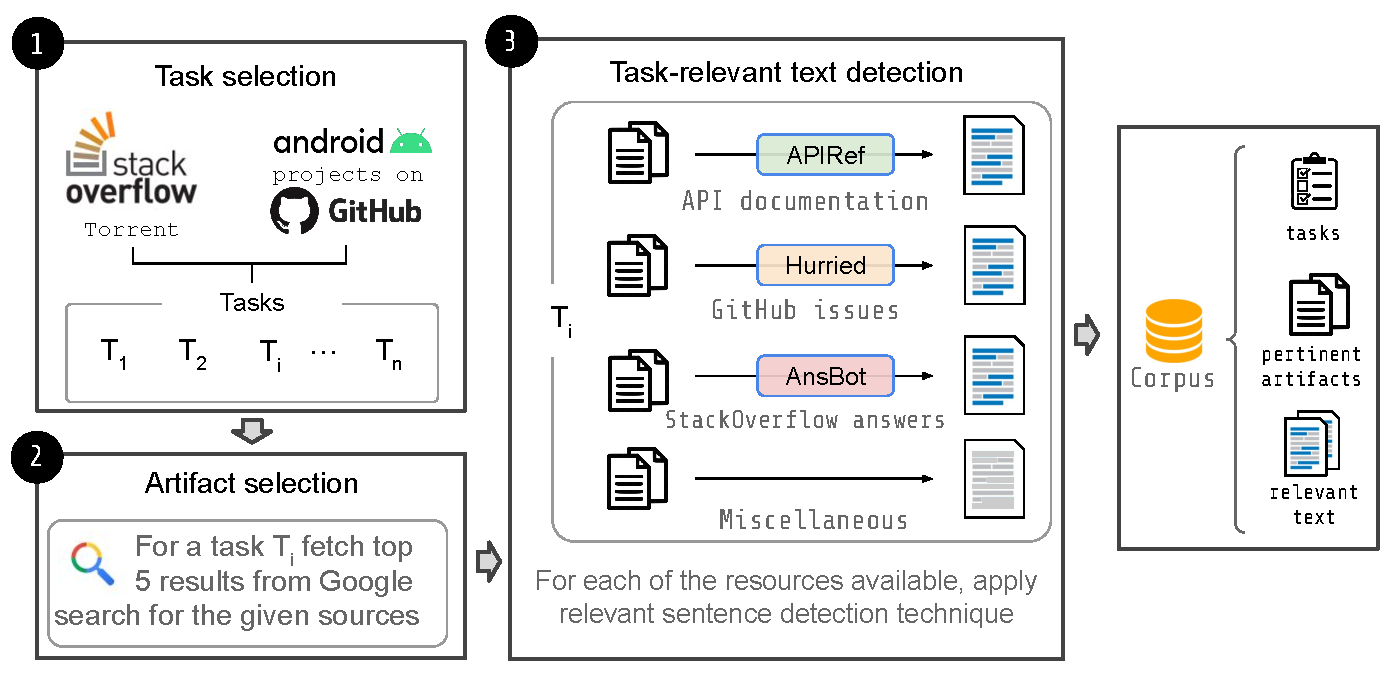
\includegraphics[width=\textwidth]{cp4/corpus-creation-pipeline}
%     \caption{Summary of procedures for corpus creation}
%     \label{fig:corpus-creation-pipeline}
% \end{figure}

